\section{Introduction}
\label{sec:introduction}

Wavetable oscillators store one period and wrap the read pointer at the end of the table.
Stored wavetables often mismatch at the wrap join ($x[0]\neq x[L{-}1]$), which can produce an audible click when the read pointer wraps; this is the seam-repair target, distinct from ordinary adjacent-sample variation within a smooth period.

\paragraph{Wavetable synthesis in brief.}
A wavetable synthesizer stores a single cycle of a waveform (the wavetable) and produces continuous tone by looping a read pointer through that table.
Pitch is set by how fast the pointer advances. Timbre comes from the stored shape (and, in multi-table banks, from morphing across tables).
Tiling the stored period yields a sustained note under playback.
When endpoints disagree, tiling places a large sample jump at the wrap join (the seam), the usual click mechanism in wavetable playback.
Figure~\ref{fig:wavetable-primer} shows one stored period, tiled playback with wrap marks, and a zoomed mismatched wrap.
The same geometry appears whenever a short loop is tiled for listening or scoring.

\begin{figure}[t]
  \centering
  \includegraphics[width=\linewidth]{figures/fig_wavetable_primer.png}
  \caption{Wavetable synthesis primer.
  (a)~One stored period $x[0..L{-}1]$ ($L{=}256$).
  (b)~The same period tiled for continuous playback. Dashed lines mark read-pointer wraps.
  (c)~Zoom at a mismatched wrap join (seam), where the endpoint cliff produces an audible click.}
  \label{fig:wavetable-primer}
\end{figure}

\paragraph{Terminology.}
Key names used below.
A \textbf{seam} (wrap join) is the local end/start junction where endpoint mismatch produces the period-locked click: the seam is local, while the signal is the whole waveform.
\textbf{Repair operator} $\Theta$ means a searchable local edit at that seam (legacy: bake cell), and a tiny network inside $\Theta$ is a \textbf{residual operator}.
\textbf{FitCell} continuously fits one candidate $\Theta$ under residual loss (Appendix~\ref{app:algorithms}).
Scores $R$ and $R_{\mathrm{blend}}$ are unsupervised: prolonged $R$ is debug-only, and $R_{\mathrm{blend}}$ drives primary selection together with the latency-aware objective $J=R_{\mathrm{blend}}-\lambda\cdot\mathrm{latency\_norm}$ (Section~\ref{sec:residual-score}).
\textbf{MoE} soft-gates bake experts, and \textbf{PBT} mutates elites in the outer loop.
The \textbf{outer loop} (meta-search) runs GA plus PPO over repair-operator graphs rather than end-to-end training of one large network.
A \textbf{holdout} freezes the evaluation set or seed for reported scores.

\paragraph{Unsupervised, as used here.}
Search does not train on paired studio-clean audio (Section~\ref{sec:eval-protocol}).
The ideal sibling $r^{\star}$ is a procedural cliff-withheld twin of the cracked engine (self-supervised geometry for scoring), not a human-labeled clean recording.
Operators are ranked under $R_{\mathrm{blend}}$ without requiring labeled clean targets at search time.

I treat the task as \emph{cycle-local seam restoration}: edit a neighborhood of the wrap join (the seam), and optionally a small residual operator over the period, so multi-period playback matches an ideal reference without the wrap cliff (Section~\ref{sec:ideal-tile}).
Agreement uses a discontinuity-weighted blend $R_{\mathrm{blend}}$ (seam fidelity vs the ideal, plus mid-cycle identity vs the cracked engine) under a latency-aware objective $J$ (Section~\ref{sec:residual-score}).

\paragraph{Four roles.}
Keep these distinct (Figure~\ref{fig:intro-sine} and Section~\ref{sec:four-roles}):
\begin{enumerate}
  \item \textbf{Ideal sibling} $r^{\star}$: cliff withheld. Scoring target only. Not a method.
  \item \textbf{No-bake}: unrepaired cracked engine $x$, scored vs $r^{\star}$. A do-nothing reference.
  \item \textbf{Dual Cosine}: classical raised-cosine end fade. Classical baseline.
  \item \textbf{Ours (DenoiseOpt)}: searched repair operator from the hybrid outer loop.
\end{enumerate}
Corrupt-to-corrupt \textbf{Noise2Noise} is a fifth comparator: the primary neural gate under the locked $R_{\mathrm{blend}}$ protocol (Section~\ref{sec:n2n-vs-ours-boards}).
It is not shown in Figure~\ref{fig:intro-sine}, which illustrates roles on one hard sine-wrap tile.

\begin{figure}[t]
  \centering
  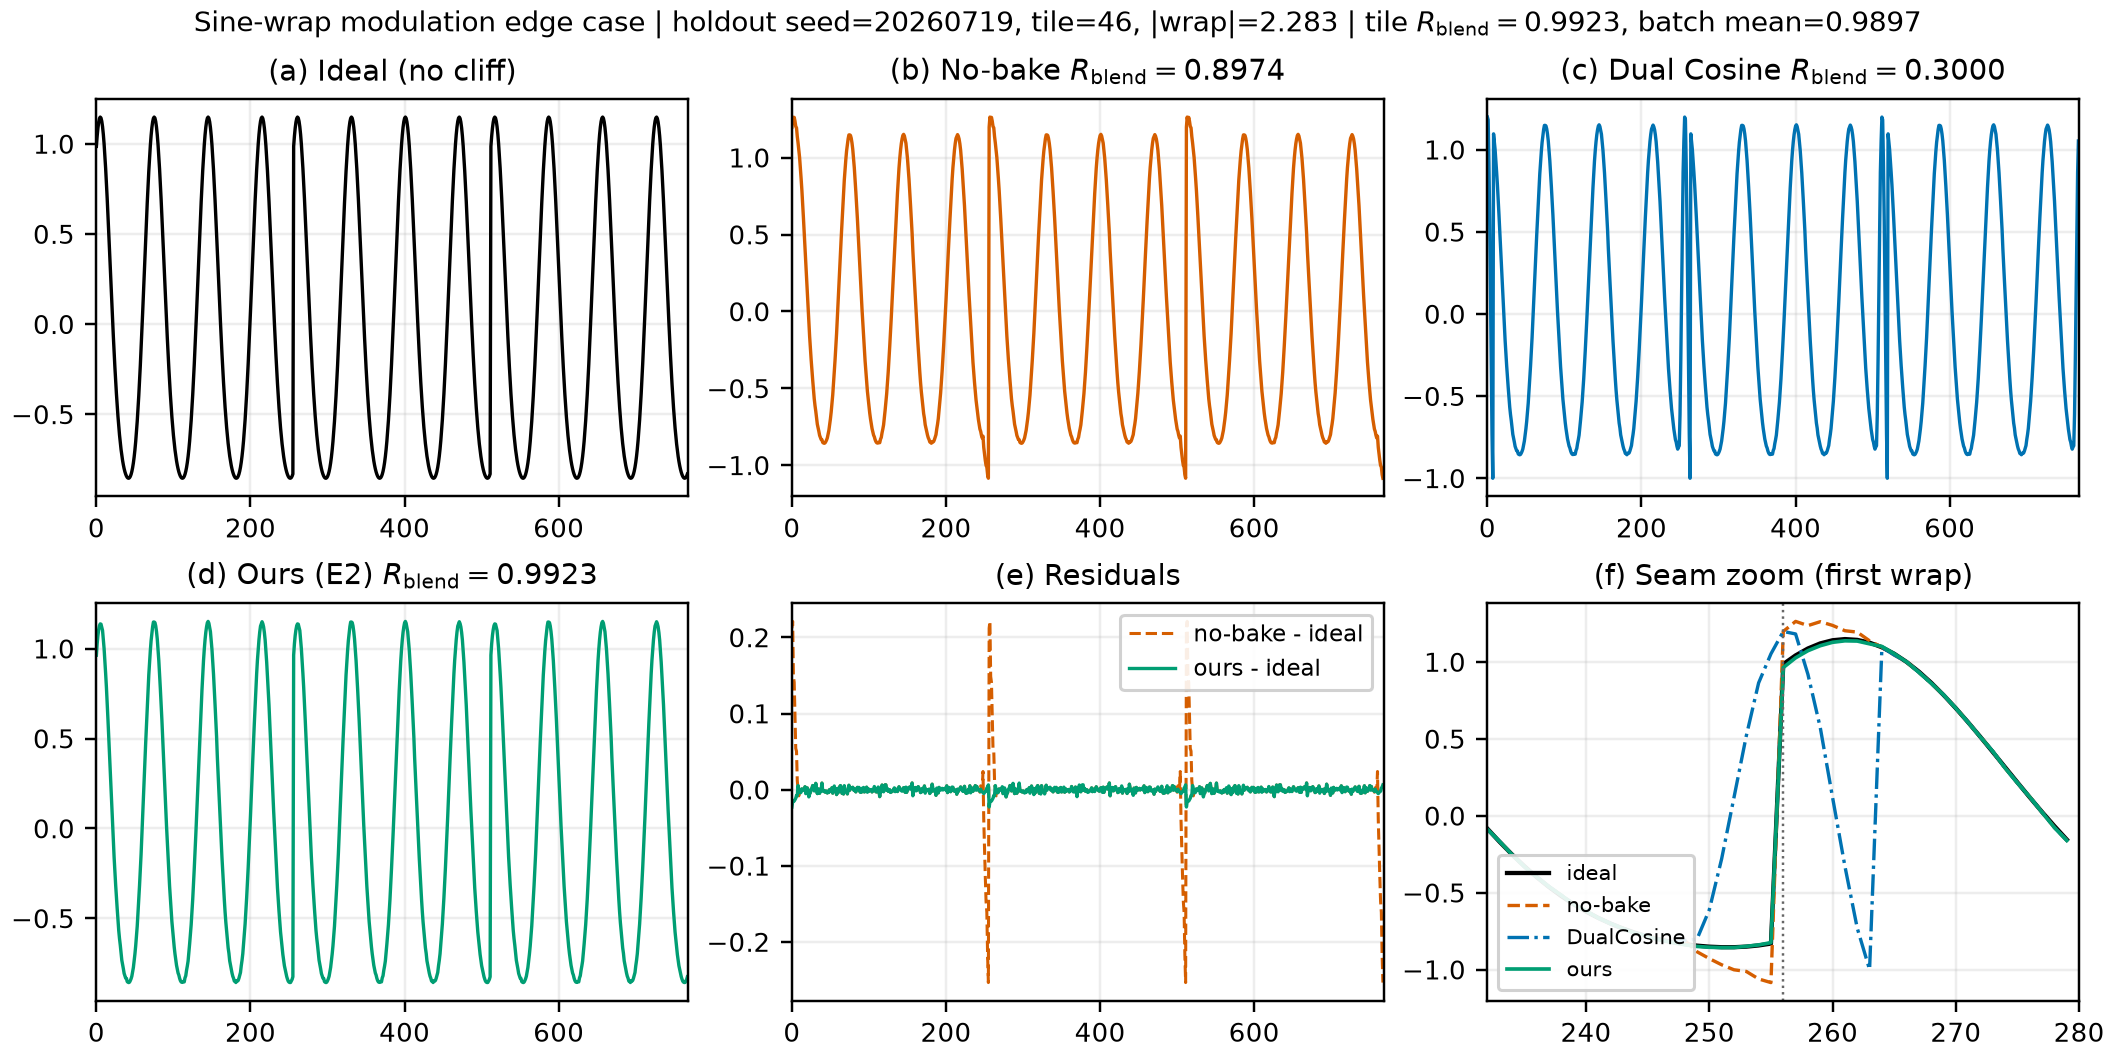
\includegraphics[width=\columnwidth]{figures/fig_intro_sine_problem.png}
  \caption{Hard sine-wrap holdout tile (seed~\texttt{20260719}).
  (a)~Ideal sibling $r^{\star}$.
  (b)~No-bake cracked engine.
  (c)~Dual Cosine fade.
  (d)~Ours (searched bake).
  (e)--(f)~Residual and seam zoom.
  Accompanying JSON scores use locked $R_{\mathrm{blend}}$ ($\alpha{=}0.7$; tile~46: no-bake $0.897$, Dual Cosine $0.300$, Ours $0.989$; Table~\ref{tab:n2n-vs-ours}).}
  \label{fig:intro-sine}
\end{figure}

Classical virtual-analog tools already address wrap energy locally
(BLIT/BLEP~\cite{stilson1996,valimaki2007polyblep}, PolyBLEP~\cite{valimaki2007polyblep}, BLAMP~\cite{esqueda2016blamp}).
I score cycle-local bake versions of those operators beside Dual Cosine (Section~\ref{sec:va-seam-baselines}).
Label-free restoration such as Noise2Noise shows that useful restorers can be trained without paired clean targets~\cite{lehtinen2018,kashyap2021n2n}; here an explicit seam geometry is what lets such reconstructors be ranked.
On the search side, I \emph{reuse} known NAS, aging evolution, PBT, CMA-ES, and PPO tools~\cite{elsken2019,real2019,jaderberg2017,hansen2016cmaes,schulman2017,khadka2018}: GA for diversity, PPO for discrete architecture edits, PBT-style exploit--mutate on elites.
The engineering choice is to combine them as an outer loop over compact seam-repair graphs. That combination is not claimed as an algorithmic contribution, and the $n{=}3$ outer-loop pilot serves solely as a compute-allocation heuristic rather than a confirmatory search-algorithm claim.

\paragraph{Key findings.}
Under the locked v10.1 $R_{\mathrm{blend}}$ protocol (objective wrap-discontinuity metrics only; no perceptual or listening claim, $N_{\mathrm{listeners}}{=}0$):
\begin{itemize}
  \item \textbf{Synthetic-cliff confirmatory (Holm--Bonferroni, Table~\ref{tab:n2n-vs-ours}):} On procedural sine+cliff holdout, E2 DenoiseOpt exceeds frozen \texttt{SeamN2N} (same protocol, \emph{not} matched training targets) on ten evaluation seeds ($0.9903{\pm}0.0010$ vs $0.9764{\pm}0.0020$, $p_{\mathrm{adj}}{=}0.0039$) and multi-family ($p_{\mathrm{adj}}{=}0.0039$).
  Factory+FX and AKWF use real cycles with \emph{injected} cliffs and per-domain search vs domain-trained N2N.
  \item \textbf{Natural real seams (negative):} Without cliff injection, no-bake beats every repair on factory and AKWF held-out cycles (Section~\ref{sec:real-natural-seam}).
  \item \textbf{Hard cliffs:} On top-$10\%$ wrap cliffs, Dual Cosine collapses ($0.9913$ edge RMSE vs $0.0944$ for \texttt{no-bake}; Table~\ref{tab:cliff-edge-rmse}).
\end{itemize}
\paragraph{Exploratory compute-allocation note.}
Under a $16$--$48$-step FitCell cap, the hybrid trails frozen Noise2Noise on $10$-seed holdout ($0.9710$ vs $0.9764$, $p{=}0.0020$); training to plateau (E2) reverses this gap.
An underpowered $n{=}3$ search-seed pilot ($0.9748{\pm}0.0018$, exact sign-flip $p{=}0.25$) motivates hybrid-only FitCell-to-plateau; it is not confirmatory superiority over outer-loop families (Section~\ref{sec:results}).
\paragraph{Scope and roadmap.}
Cycle-local wavetable seam repair for DSP and synthesis venues; formal wrap-closure proofs, search-convergence theorems, and human perceptual trials ($N_{\mathrm{listeners}}{=}0$) are out of scope (Section~\ref{sec:limitations}).
Section~\ref{sec:methods} defines $R_{\mathrm{blend}}$, $J$, and the operator space; Section~\ref{sec:experiments} details datasets and baselines; Section~\ref{sec:results} presents confirmatory, ablation and sensitivity results; exploratory cross-domain checks are in the appendix.

\subsection{Contributions}
\label{sec:contributions}
\begin{enumerate}
  \item \textbf{Problem framing.} Wrap discontinuity as cycle-local seam restoration under tiled evaluation, with explicit $R_{\mathrm{seam}}$, $R_{\mathrm{body}}$, and primary locked $R_{\mathrm{blend}}$ ($\alpha{=}0.7$) plus latency-aware $J$.
  \item \textbf{Ideal-sibling protocol.} Unsupervised scoring via a procedural cliff-withheld twin plus mid-cycle engine identity, without paired studio-clean targets at search time.
  \item \textbf{Compact repair-operator space.} Searchable graphs over classical seam ops (DualCosine, FIR, VA residuals) and tiny residual nets (MLP/FIR/U-Net-lite/LSTM-lite/MoE), not end-to-end Demucs-scale stacks (Section~\ref{sec:bake}, Appendix~\ref{app:algorithms}).
  \item \textbf{Engineering instantiation (not an algorithmic claim).} DenoiseOpt reuses standard GA--PPO(+PBT) primitives as an outer loop over that operator space; an exploratory $n{=}3$ six-way $5$k pilot ($p{=}0.25$) serves solely as a compute-allocation heuristic for FitCell-to-plateau (Tables~\ref{tab:meta-approaches},~\ref{tab:v14-hybrid-converge}).
  \item \textbf{Open multi-seed, multi-family, and cross-domain evaluation.} A frozen \texttt{SeamN2N} neural baseline, $10$-seed holdout, multi-family and wavetable-native boards, hard-cliff strata, and exploratory 7-domain engineering transfer checks (Section~\ref{sec:ethics}, Appendix~\ref{app:transfer-bundle}).
\end{enumerate}
What is \emph{not} claimed as a contribution: a new foundational NAS/RL algorithm, formal wrap-closure theorems, or perceptual MOS/MUSHRA superiority.
